\chapter{Results}
\label{cha:results}
This \namecref{cha:results} covers the results from running our
implementation (\cref{cha:implementation}) for the algorithm presented
in \cref{cha:mmlt} on a uniform distribution of random points in the
unit square.
%\section{Technical Details}
All experiments were run on an Intel\textsuperscript{\textregistered}~%
Core\texttrademark~2 Duo CPU E6850 with 2 GB RAM. For everything but
the IP-solving with CPLEX only one core is used. We compiled with the
GCC 4.7.2 and following options: \verb|-frounding-math -std=c++11 -O3|.
The libraries we compiled against are Qt 5.0.0, CGAL 4.0.2, Boost 1.49,
and JSON Spirit 4.06.

\section{Segment Lengths}
\label{sec:results_segments}
Our first experiments were made to verify \cref{thm:index_enose} by
computing the Edge Length Index of the Shortest Non-separable Edge
\(\idx(\gls{enose})\) for various numbers of input points.
\Cref{fig:segment_length,fig:segment_index} show the trend of
\gls{enose} in comparison with the shortest line segment, and
with the minimum Edge Length Index of the \gls{MELT} solution, respectively.
For each data point 100 instances were run, though some of them have
been aborted after 30 minutes
(refer to \cref{tab:segment_index,tab:segment_length}).

Even though the specific progression of the Shortest Non-separable
Edge index \(\idx(\gls{enose})\) is not clear from \cref{fig:segment_index}, it can be
assumed that it is sub-linear. From \cref{fig:segment_length}, we can
also see that the shortest line segment length significantly drops below
the length of \gls{enose}, which results in more
segments being in between for a uniform distribution.

\section{Execution Time}
Furthermore, we made an analysis of our algorithm's running time
with respect to the number of input points. Again we let 100 instances 
run for each data point. The resulting times are real time (in contrast 
to user or system time)---i.e. execution time of non-related background 
processes is not excluded. This decision was made because it is usually 
impossible to guarantee that no other (system) tasks are running, so real 
time is more meaningful (yet less accurate).

\Cref{fig:time_composition} shows which part of our algorithm takes
what amount of time in comparison to the full execution execution
time. As can be seen, generating the Complete Graph and sorting the
line segments by Edge Length Order takes polynomial time (red bars).
The high variance in the time for \gls{IP} solving (blue) is due to
heuristics being used in CPLEX to reduce the exponential worst case
running time. All remaining parts of the algorithm, including
constructing of the Intersection Graph, and computing the Constrained
Point Set Triangulation take significantly less time (green). By now,
we can not explain the gap for 470 to 490 input points. For the
complete data refer to \cref{tab:time_composition}.

For a comparison in terms of running time of our algorithm versus
solving the complete \gls{MELT} instance as an \gls{IP}
(involving the construction of a complete Intersection Graph) see
\cref{fig:time_total}. For the data points, we use the median of all
running times combined with the median absolute deviation. As
\cref{fig:time_hist} shows, we have to deal with heavy outliers
starting at a problem size of 80 input points, which is why we chose
to use median instead of average.

\section{Aborted instances}
\label{sec:aborted_instances}
As you will have noticed in \cref{fig:time_total}, there are only few
data points, and also in \cref{cha:result_data} there are some cases
where not all 100 instances are part of the table. This is because
we aborted every instance after exceeding a running time of 30
minutes. See \cref{fig:time_hist_num} for an impression on how many
instances could be completed within a certain time (here 23 minutes
and 20 seconds).

%---------------------------------------------------------------------##########

\begin{landscape}
\begin{figure}[ht]
  \centering
  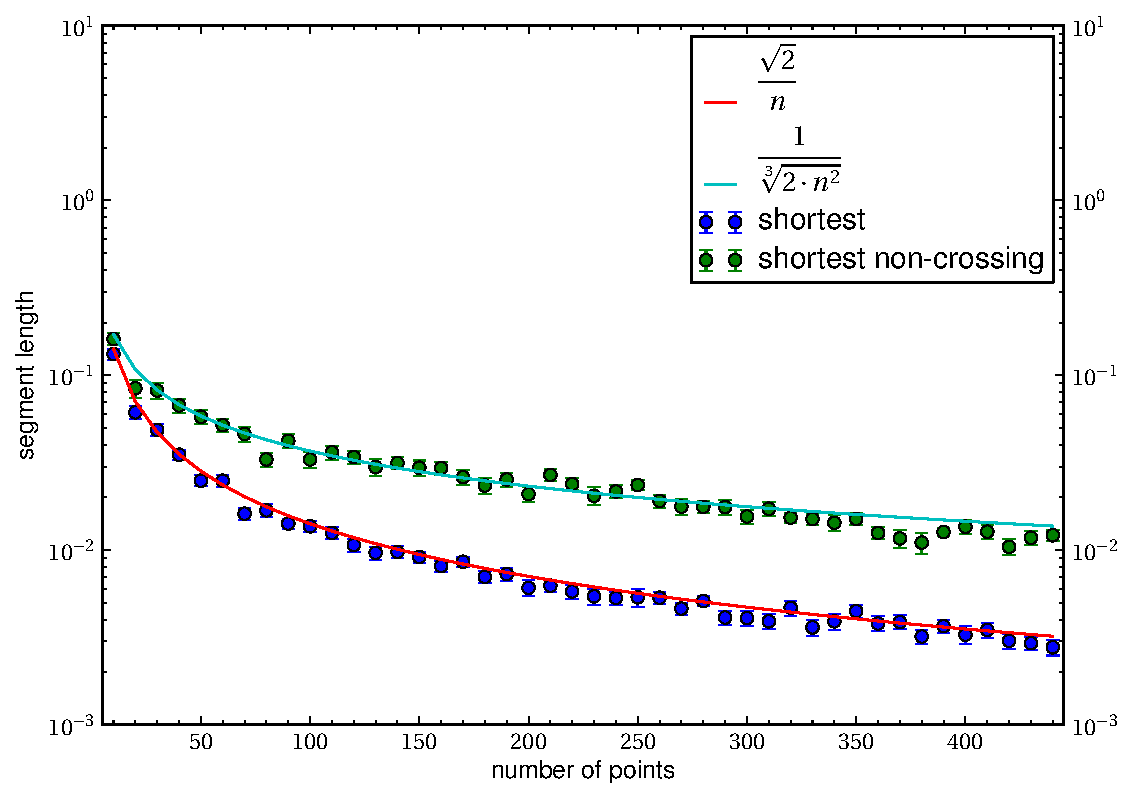
\includegraphics[width=\linewidth,keepaspectratio]{results/segment_length.pdf}
  \caption{\label{fig:segment_length}Comparison of segment lengths}
\end{figure}

\begin{figure}[ht]
  \centering
  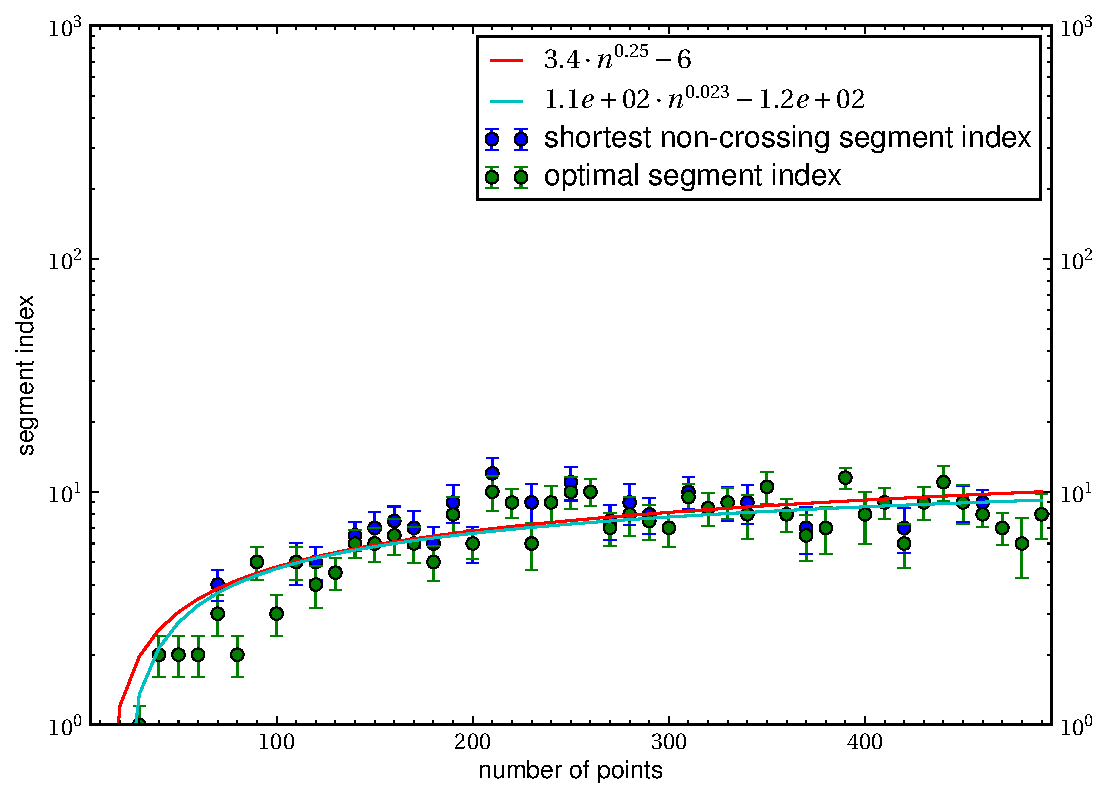
\includegraphics[width=\linewidth,keepaspectratio]{results/segment_index.pdf}
  \caption{\label{fig:segment_index}Comparison of segment indices}
\end{figure}
\end{landscape}

%\newgeometry{margin=1.5cm}
%\begin{landscape}
\begin{figure}[ht]  
  \begin{minipage}{\textwidth}
  \centering
  %\thisfloatpagestyle{empty}
  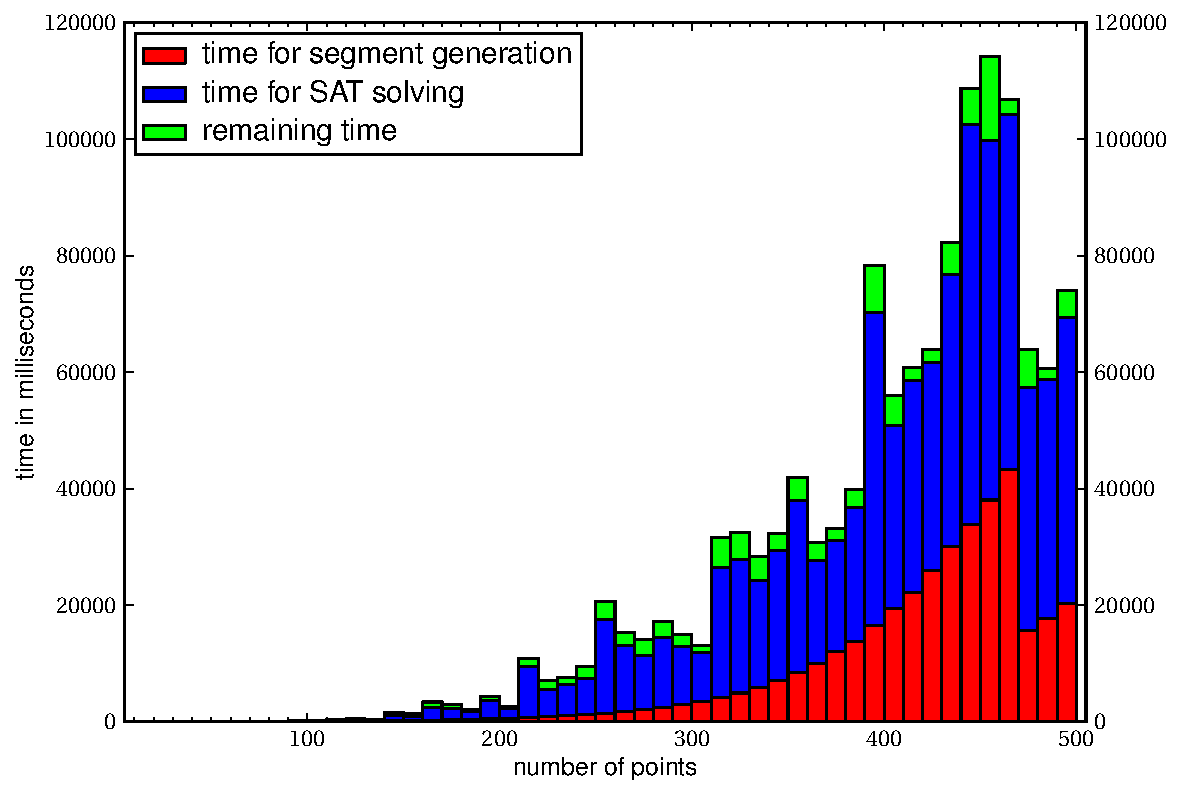
\includegraphics
  [width=\linewidth,height=\textheight,keepaspectratio]
  {results/time_composition.pdf}
  \caption[Composition of execution times]
  {\label{fig:time_composition}Composition of execution times%
    \footnote[0]{* is where the magic happens: we currently can not explain this gap}
  }
  \end{minipage}
\end{figure}
%\end{landscape}
%\restoregeometry

\begin{figure}[ht]
  \centering
  \begin{subfigure}{\textwidth}
    \centering
    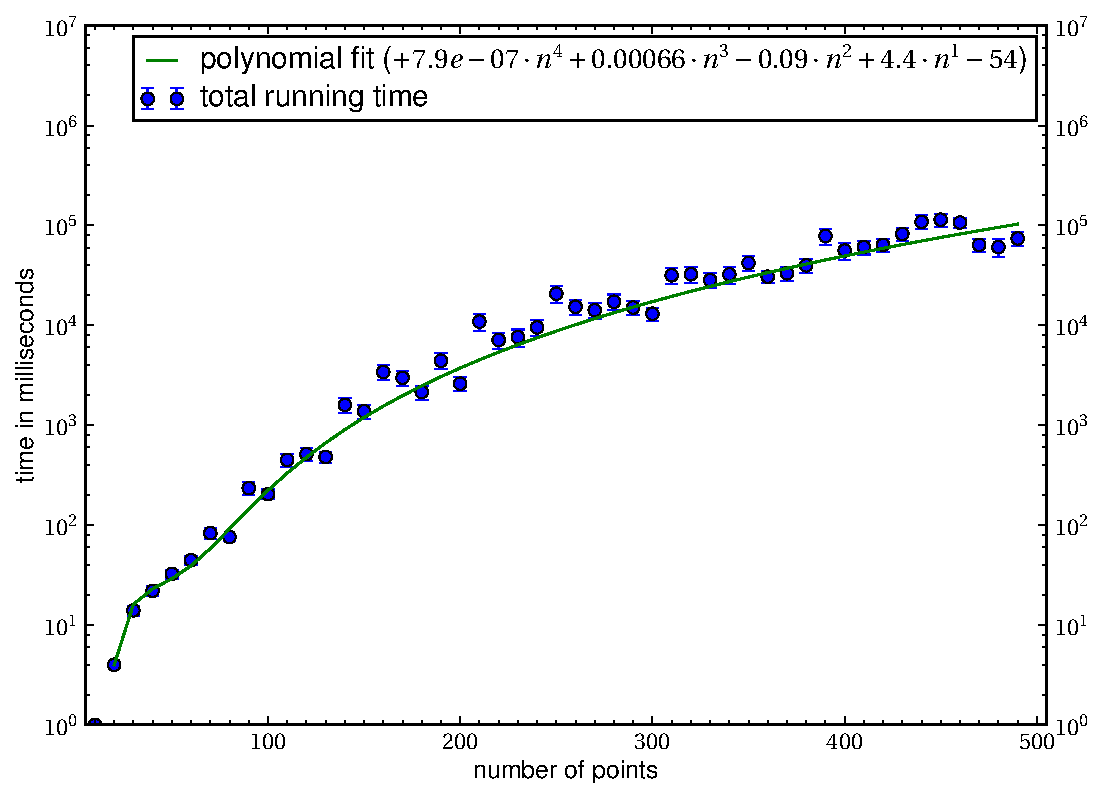
\includegraphics
    [width=\linewidth,height=\textheight,keepaspectratio]
    {results/time_total.pdf}
    \caption{Our Algorithm}
  \end{subfigure}
  
  \begin{subfigure}{\textwidth}
    \centering
    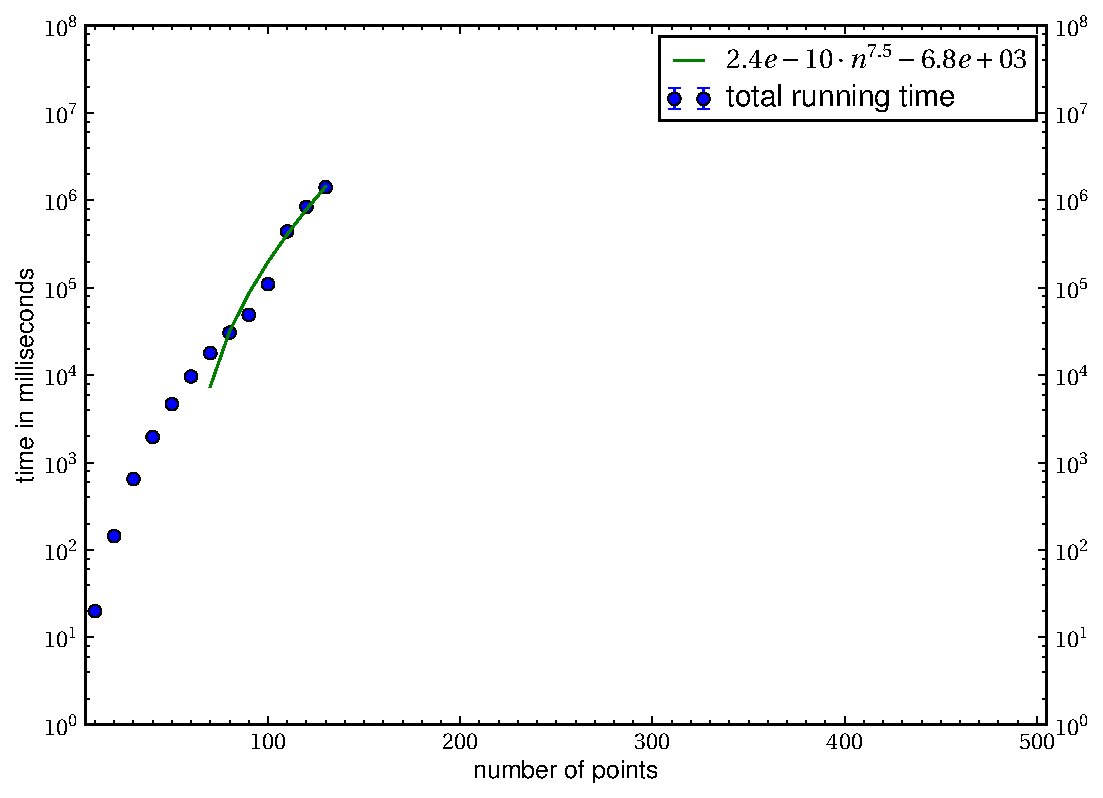
\includegraphics
    [width=\linewidth,height=\textheight,keepaspectratio]
    {results/complete_sat/time_total.pdf}
    \caption{Complete Intersection Graph and \gls{IP}}
  \end{subfigure}
  \caption{\label{fig:time_total}Total execution time}
\end{figure}

\begin{figure}[ht]
  \centering
  \begin{subfigure}{\textwidth}
    \centering
    \includegraphics%
    [width=\linewidth,height=\textheight,keepaspectratio]
    {results/time_hist_0070.pdf}
    \caption{\label{fig:times_70}70 points}
  \end{subfigure}
  
  \begin{subfigure}{\textwidth}
    \centering
    \includegraphics%
    [width=\linewidth,height=\textheight,keepaspectratio]
    {results/time_hist_0080.pdf}
    \caption{\label{fig:times_80}80 points}
  \end{subfigure}
  \caption{\label{fig:time_hist}Histogram of execution times}
\end{figure}

%\newgeometry{margin=1.5cm}
%\begin{landscape}
\begin{figure}[ht]
  \centering
  \begin{subfigure}{\textwidth}
    \centering
    \includegraphics%
    [width=\linewidth,height=0.4\textheight,keepaspectratio]%
    {results/complete_sat/time_hist.pdf}
    \caption{Complete SAT}
  \end{subfigure}
  
  \begin{subfigure}{\textwidth}
    \centering
    \includegraphics%
    [width=\linewidth,height=0.4\textheight,keepaspectratio]%
    {results/time_hist.pdf}
    \caption{Improved method}
  \end{subfigure}
  \caption{\label{fig:time_hist_num}Instances with running time < 23:20min}
\end{figure}
%\end{landscape}
%\restoregeometry

%---------------------------------------------------------------------##########
